%======================================================================
\NEWSEC
%======================================================================

\subsection{\ssRecentCosmology}

\begin{frame}[fragile,label=ss-recent-cosmology] 
\secframetitle{\ssRecentCosmology}
\begin{itemize}
\item Block size $32^3$
\end{itemize}
\begin{center}
\begin{minipage}{2.0in}
\only<1->{\ANIMATEGRAPHICS{width=2.0in}{05}{Images/Comet-run.34/dark-}{00}{33}}
\end{minipage} \ 
\begin{minipage}{2.0in}
\only<1->{\ANIMATEGRAPHICS{width=2.0in}{05}{Images/Comet-run.34/mesh-}{00}{33}}
\end{minipage}
\end{center}
\end{frame}

%----------------------------------------------------------------------

\begin{frame}[fragile,label=ss-recent-cosmology] 
\secframetitle{\ssRecentCosmology}
\begin{itemize}
\item Block size $16^3$
\end{itemize}
\begin{center}
\begin{minipage}{2.0in}
\only<1->{\ANIMATEGRAPHICS{width=2.0in}{05}{Images/Comet-run.35/dark-}{00}{26}}
\end{minipage} \ 
\begin{minipage}{2.0in}
\only<1->{\ANIMATEGRAPHICS{width=2.0in}{05}{Images/Comet-run.35/mesh-}{00}{26}}
\end{minipage}
\end{center}
\end{frame}

%----------------------------------------------------------------------


\begin{frame}[fragile,label=ss-recent-cosmology] 
\secframetitle{\ssRecentCosmology}
\begin{itemize}
\item Block size $8^3$
\end{itemize}
\begin{center}
\begin{minipage}{2.0in}
\only<1->{\ANIMATEGRAPHICS{width=2.0in}{05}{Images/Comet-run.36/dark-}{00}{21}}
\end{minipage} \ 
\begin{minipage}{2.0in}
\only<1->{\ANIMATEGRAPHICS{width=2.0in}{05}{Images/Comet-run.36/mesh-}{00}{21}}
\end{minipage}
\end{center}
\end{frame}


\begin{frame}[fragile,label=ss-recent-cosmology] 
\secframetitle{\ssRecentCosmology}
\centerline{Block size $32^3$ runs the fastest}
\begin{center}
\begin{minipage}{3.5in}
\only<1->{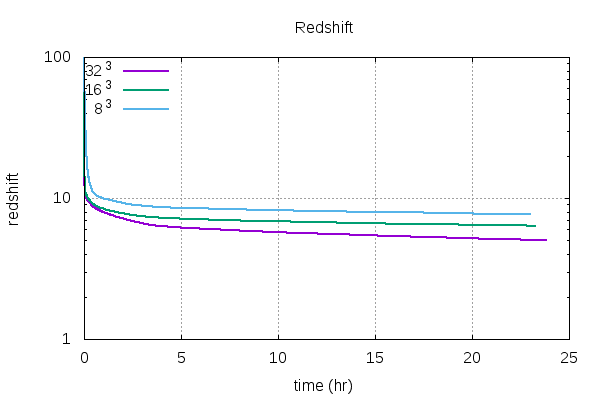
\includegraphics[width=3.5in]{Images/b345-redshift.png}}
\end{minipage} \ 
\end{center}
\end{frame}

\begin{frame}[fragile,label=ss-recent-cosmology] 
\secframetitle{\ssRecentCosmology}
\centerline{But block size $32^3$ uses the most memory}
\begin{center}
\begin{minipage}{3.5in}
\only<1->{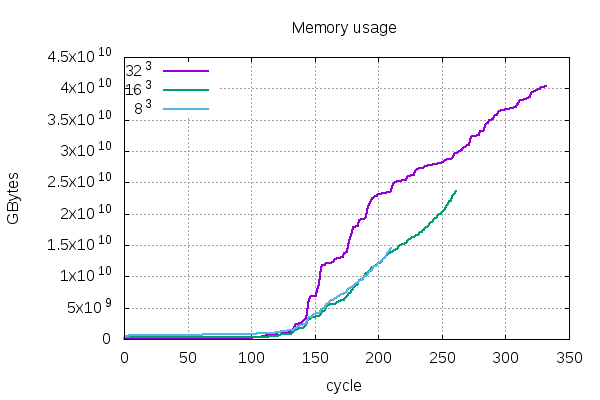
\includegraphics[width=3.5in]{Images/b345-bytes.png}}
\end{minipage} \ 
\end{center}
\end{frame}

\begin{frame}[fragile,label=ss-recent-cosmology] 
\secframetitle{\ssRecentCosmology}
\centerline{Time per cycle has a burst of growth at varying points}
\begin{center}
\begin{minipage}{3.5in}
\only<1->{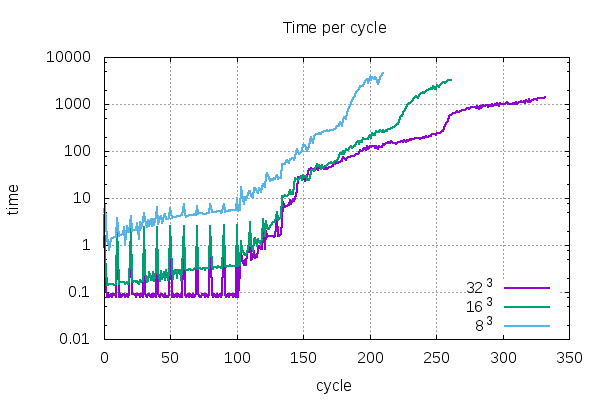
\includegraphics[width=3.5in]{Images/b345-time-per-cycle-log.png}}
\end{minipage}
\end{center}
\end{frame}

\begin{frame}[fragile,label=ss-recent-cosmology] 
\secframetitle{\ssRecentCosmology}
\centerline{Solver time scaled by number of blocks shows this even more}
\begin{center}
\begin{minipage}{3.5in}
\only<1->{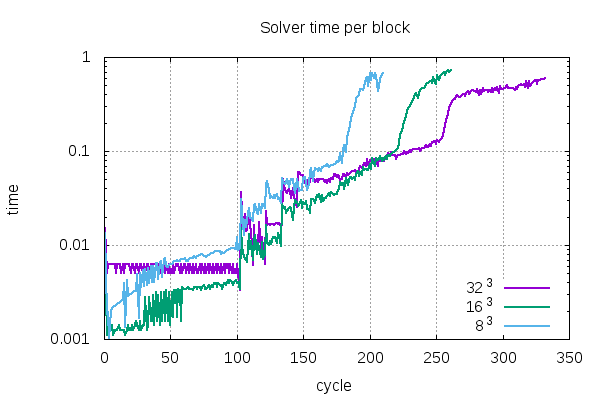
\includegraphics[width=3.5in]{Images/b345-time-per-block.png}}
\end{minipage}
\end{center}
\end{frame}

\begin{frame}[fragile,label=ss-recent-cosmology] 
\secframetitle{\ssRecentCosmology}
\centerline{Yet number of solver iterations is very reasonable}
\begin{center}
\begin{minipage}{3.5in}
\only<1->{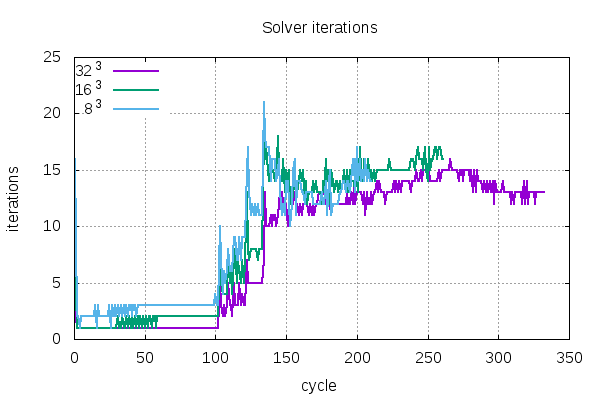
\includegraphics[width=3.5in]{Images/b345-bcg-iters.png}}
\end{minipage}
\end{center}
\end{frame}

\begin{frame}[fragile,label=ss-recent-cosmology] 
\secframetitle{\ssRecentCosmology}
\centerline{Memory per block is also increasing}
\begin{center}
\begin{minipage}{3.5in}
\only<1->{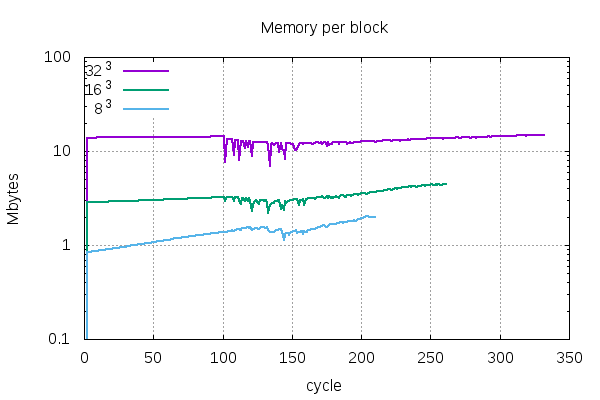
\includegraphics[width=3.5in]{Images/b345-bytes-per-block.png}}
\end{minipage}
\end{center}
\end{frame}

% \begin{frame}[fragile,label=ss-recent-cosmology] 
% \secframetitle{\ssRecentCosmology}
% Cosmological parameters are set in the \code{Physics} parameter group.
% \small
% \begin{tabbing}
% \code{xxx}\=\code{xxx}\=\code{xxx}\=\code{xxxxxxxxxxxxxxxxxxxxx}\=\kill
% \>\code{Physics \{ } \\
% \> \> \code{list = ["cosmology"];} \\
% \> \> \code{cosmology \{ } \\
% \>\>\> \code{hubble\_constant\_now} \> \code { = 0.701; } \\
% \>\>\> \code{omega\_matter\_now} \> \code{ =   0.279; } \\
% \>\>\> \code{omega\_dark\_matter\_now} \> \code { =   -1.0; } \\
% \>\>\> \code{omega\_lambda\_now} \> \code { =   0.721; } \\
% \>\>\> \code{comoving\_box\_size} \> \code { = 64.0; } \\
% \>\>\> \code{max\_expansion\_rate} \> \code { = 0.01; } \\
% \>\>\> \code{initial\_redshift} \> \code { =  20.0; } \\
% \>\>\> \code{final\_redshift} \> \code { =  0.0; } \\
% \>\>  \code{ \} } \\
% \>  \code{ \} }
% \end{tabbing}
% \end{frame}

% ----------------------------------------------------------------------


% \begin{frame}[fragile]
% \secframetitle{\ssRecentCosmology}
% Cosmological parameters are stored in an \code{EnzoPhysicsCosmology} object.
% \footnotesize
% \begin{tabbing}
% \code{xxx}\=\code{xxx}\=\code{xxxxxxxxxxxxxxxxxxx}\=\kill
% \> \code{EnzoPhysicsCosmology * cosmology = (EnzoPhysicsCosmology * )} \\
% \> \> \code{      simulation()->problem()->physics("cosmology");} \\
% \\ 
% \> \code{enzo\_float omega\_lambda\_now =} \\
% \>\> \code{cosmology->omega\_lambda\_now()} \\
% \> \code{enzo\_float time\_begin =} \\
% \>\> \code{cosmology->initial\_time\_in\_code\_units();} \\
% \\
% \> \code{cosmology->compute\_expansion\_factor (\&a,\&dadt, time);} \\
% \> \code{cosmology->compute\_expansion\_timestep (\&dt\_expansion, time);} \\ 
% \> \code{cosmology->get\_units (\&density\_units,} \\
% \>\>\> \code{\&length\_units,} \\
% \>\>\> \code{\&temperature\_units,} \\
% \>\>\> \code{\&time\_units,} \\
% \>\>\> \code{\&velocity\_units,} \\
% \>\>\> \code{time);}
% \end{tabbing}
% \end{frame}

